% Results and analysis section for OrbitGraph paper.
% Figures live in figures/ (sibling of this file; underscore filenames).

\section{Results and Analysis}
\label{sec:analysis}

We analyze the scaling study ($5{\times}5$–$10{\times}10$, ten repetitions per
grid and mode) along four axes: data-plane availability at GSL handover,
phase-resolved reachability and latency, control-plane cost, and behavior under
satellite failure.
Unless noted, handover plots aggregate the \emph{first} GSL handover in each
run so that statistics are not diluted by late-emulation events near teardown.

\subsection{Data-plane availability at GSL handover}
\label{sec:analysis-handover}

\begin{figure}[!t]
  \centering
  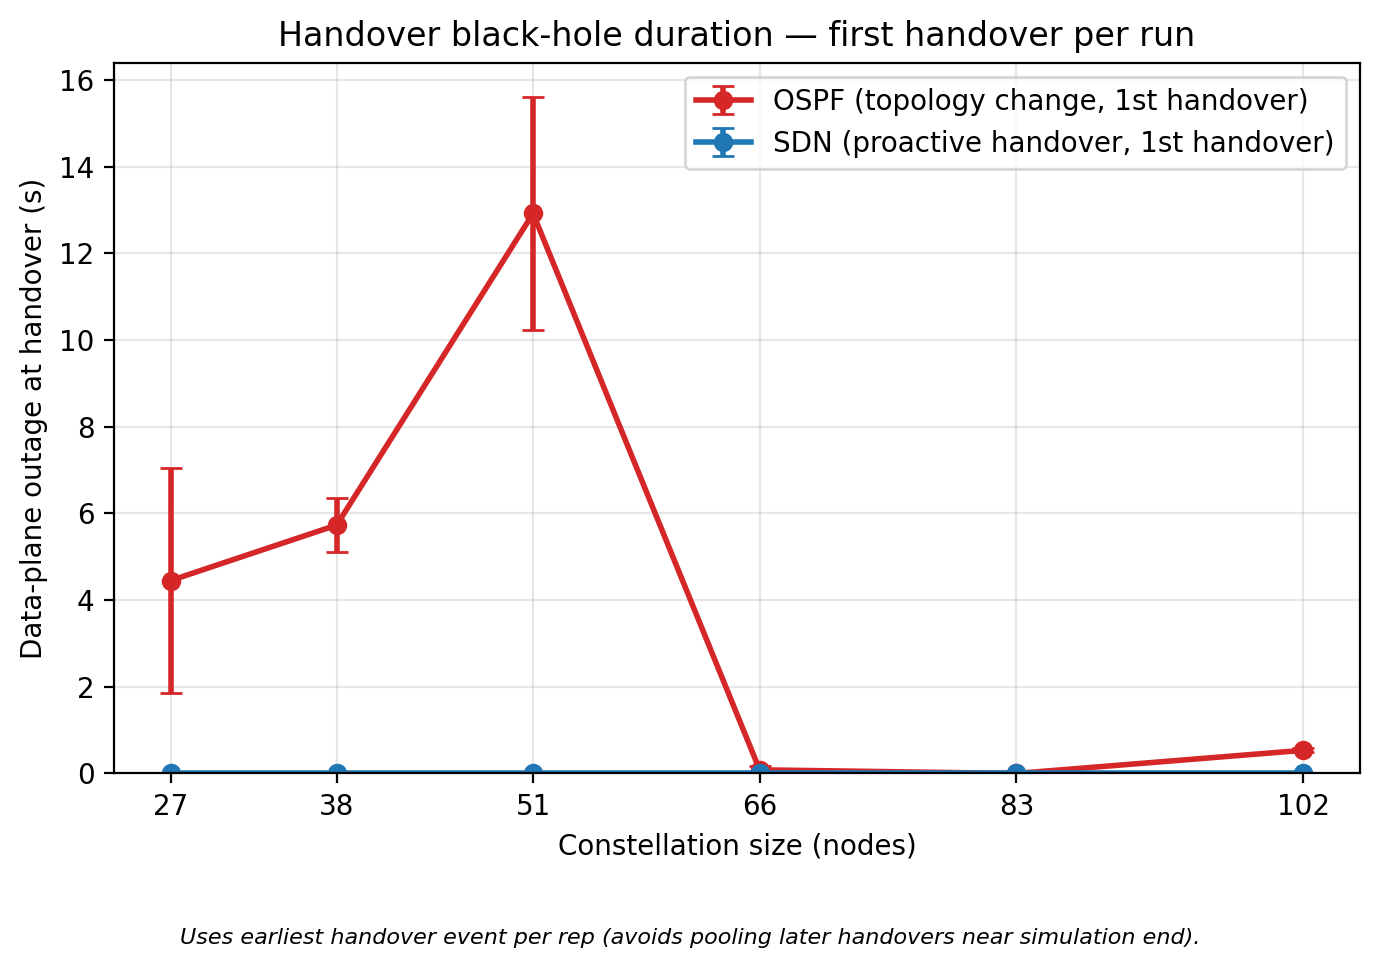
\includegraphics[width=\linewidth]{figures/outage_vs_nodes.png}
  \caption{Mean data-plane outage at the first GSL handover versus constellation
    size ($N$ nodes).
    OSPF (\texttt{topology\_change}) exhibits multi-second black holes;
    OrbitGraph (\texttt{proactive\_handover}) maintains 0\,s mean outage on every
    grid where the first handover completes inside the emulation window.
    Error bars: standard deviation over ten repetitions.}
  \label{fig:outage-handover}
\end{figure}

Figure~\ref{fig:outage-handover} is the central result of this work.
A continuous \texttt{ping} probe inside the source ground-station container
measures sustained loss bursts aligned to control-plane events
(Section~\ref{sec:experiments}); this metric captures downtime that tick-scheduled
pings miss when route installation blocks the emulation loop.

At the first handover, OSPF data-plane outage grows with constellation size and
peaks at ${\sim}13.6$\,s on the $7{\times}7$ grid (51 nodes), with
${\sim}5.7$\,s on $6{\times}6$ (38 nodes) and ${\sim}7.7$\,s on $10{\times}10$
(102 nodes).
These gaps correspond to the interval between GSL teardown and BIRD/OSPF
reconvergence---traffic is forwarded along stale or missing next-hops until
link-state flooding completes~\cite{sidhu:ospf:1993}.

OrbitGraph inverts this picture.
By installing the post-handover FIB after new GSLs are added but \emph{before}
old links are removed (Section~\ref{sec:proactive}), proactive handover yields
\textbf{0\,ms mean outage} on every grid from 27 to 102 nodes, with zero
\texttt{still\_down} events across all 60 SDN repetitions in the handover
cohort.
The data plane stays up even though the Docker-based install itself takes
seconds (Section~\ref{sec:analysis-control}): make-before-break at the topology
level, not merely at the route-entry level, is what eliminates the black hole.

This is the regime where graph-centric SDN \emph{excels}: GSL handover times
are known from orbital mechanics, the post-handover graph $G_t$ is available in
the delay matrix before the old contact is torn down, and a centralized
controller can commit forwarding for the new graph while both contacts briefly
coexist---something distributed OSPF cannot do without protocol
extensions~\cite{pam:opspf:2019,gregory:satellite-routing:2022}.

\subsection{Reachability and latency across handover phases}
\label{sec:analysis-dataplane}

\begin{figure*}[!t]
  \centering
  \begin{minipage}[t]{0.48\textwidth}
    \centering
    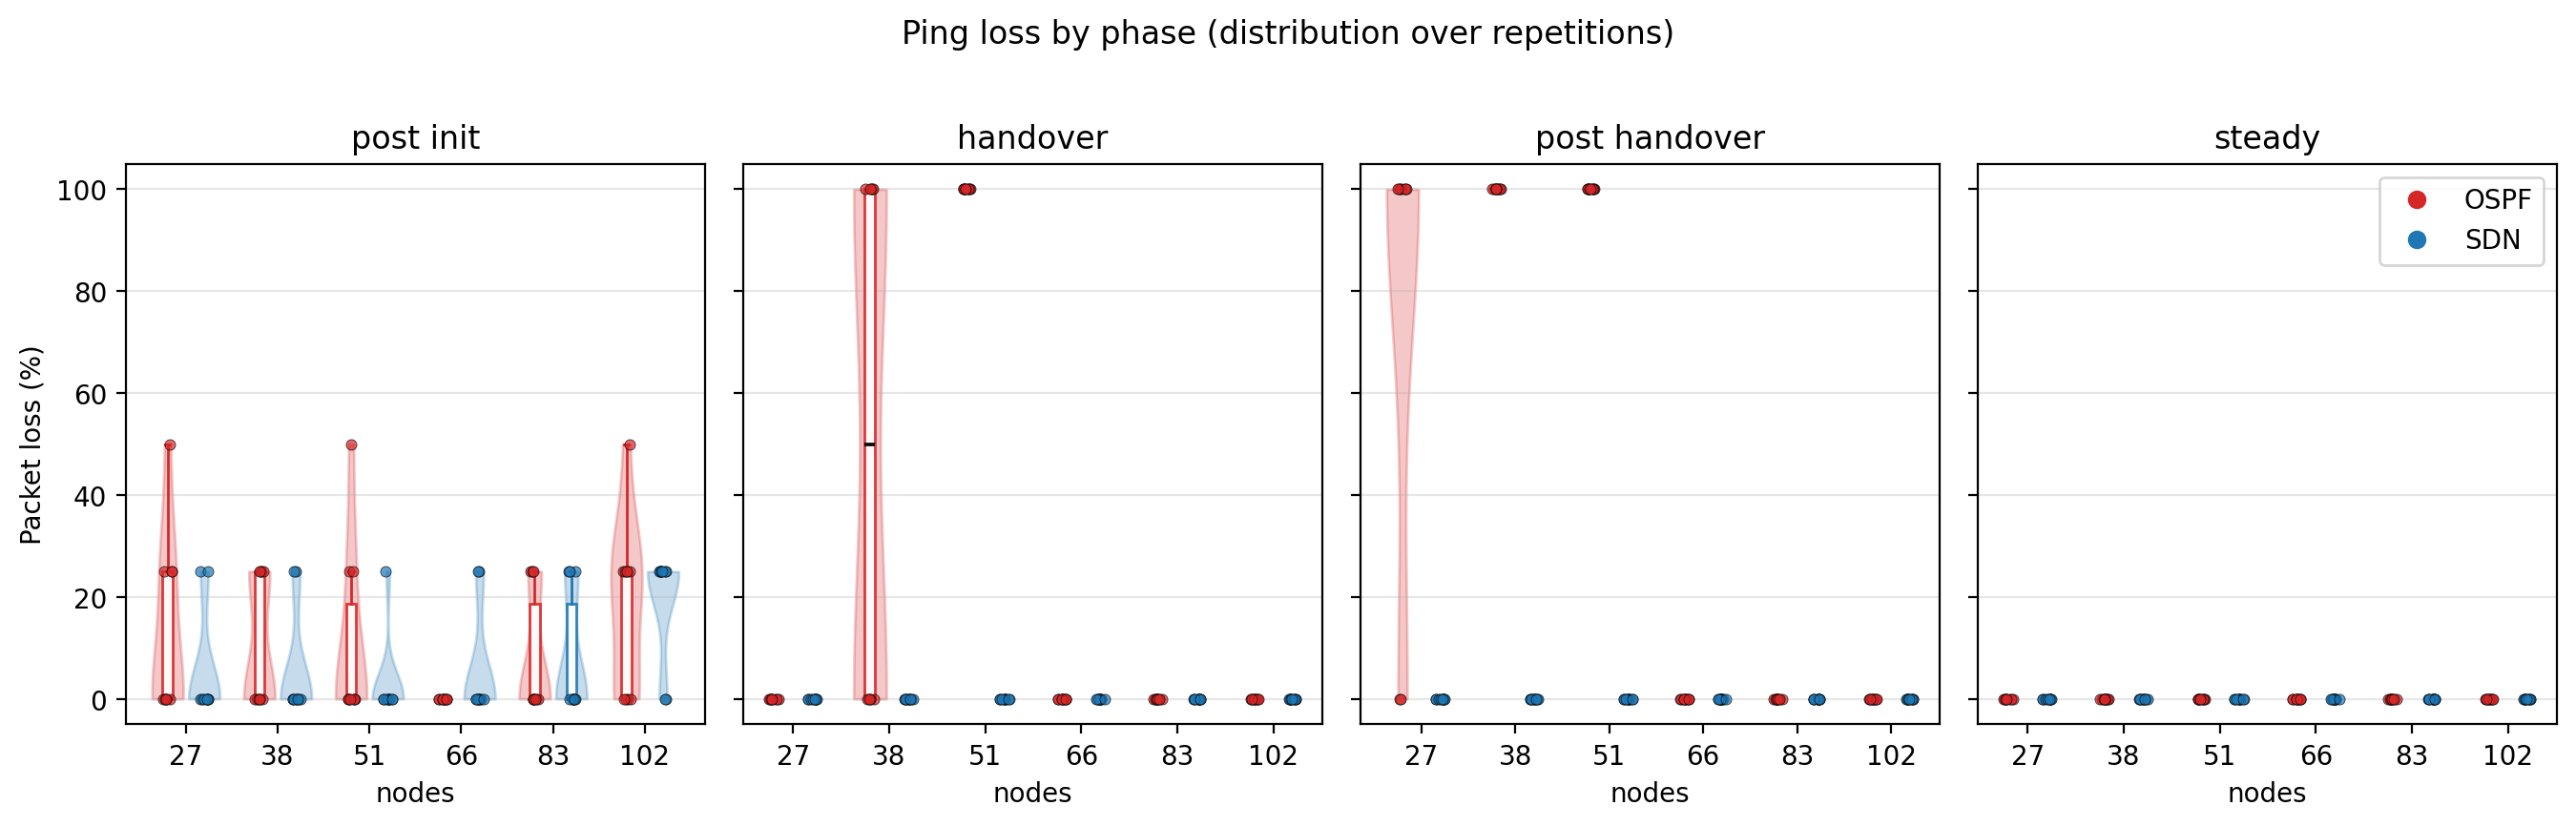
\includegraphics[width=\linewidth]{figures/loss_by_phase.png}\\[-0.5ex]
    {\footnotesize (a) Packet loss by phase}
  \end{minipage}\hfill
  \begin{minipage}[t]{0.48\textwidth}
    \centering
    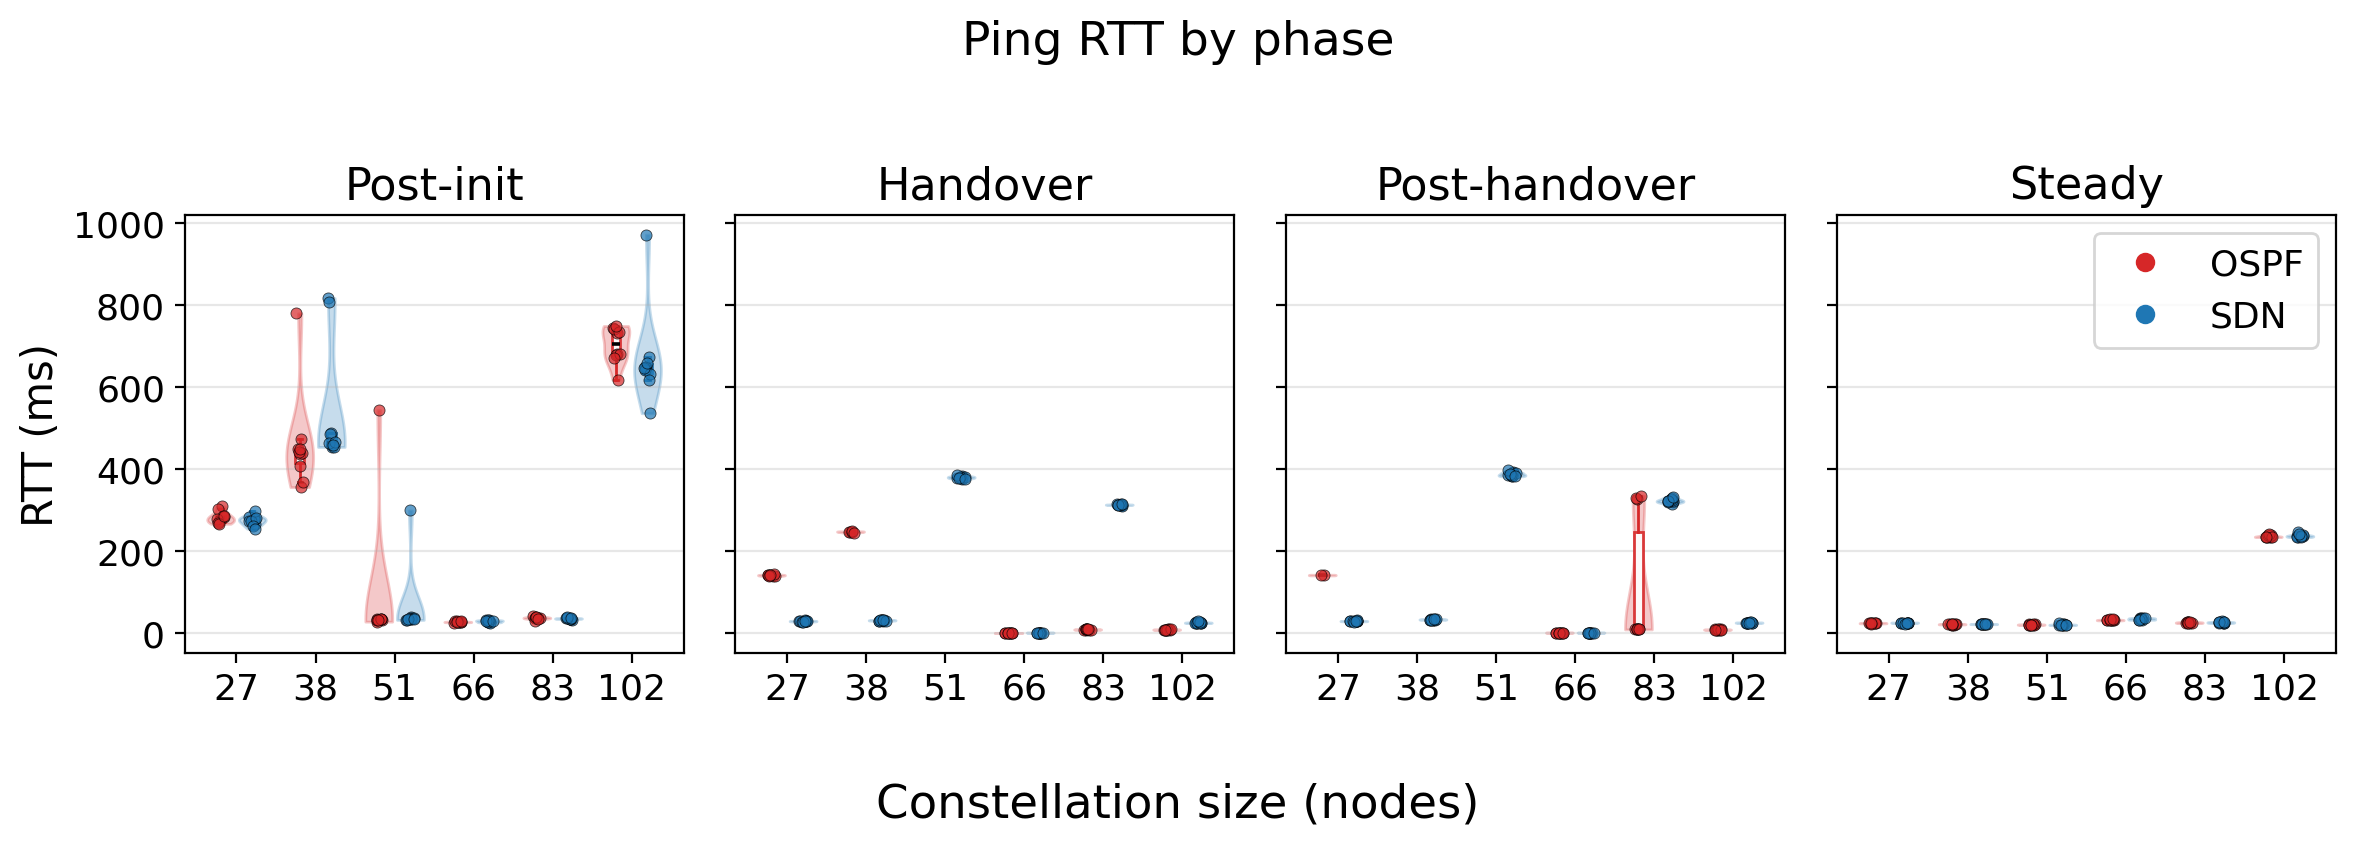
\includegraphics[width=\linewidth]{figures/rtt_by_phase.png}\\[-0.5ex]
    {\footnotesize (b) Mean RTT by phase}
  \end{minipage}
  \caption{End-to-end ground-station ping metrics by handover-relative phase
    (mean~$\pm$~stddev over ten repetitions).
    (a)~Loss; (b)~RTT.
    OrbitGraph holds 0\% loss through \texttt{handover} and \texttt{post\_handover}
    on all grid sizes; OSPF loss spikes during reconvergence (e.g., 100\% on
    $7{\times}7$).}
  \label{fig:phase-metrics}
\end{figure*}

Figure~\ref{fig:phase-metrics} complements
Figure~\ref{fig:outage-handover} with scheduled probes at the handover tick,
two seconds later, and near emulation end.

\paragraph{Packet loss.}
OrbitGraph achieves \textbf{0\% mean loss} in the \texttt{handover} and
\texttt{post\_handover} phases on every grid size.
OSPF loss is highly phase-dependent: on $6{\times}6$ half of handover probes
are lost (50\% mean); on $7{\times}7$ both handover and post-handover phases
reach 100\% loss because the path is black-holed until OSPF settles.
After convergence (\texttt{steady}), OSPF recovers to 0\% loss---both modes
eventually forward correctly once the distributed database catches up.

\paragraph{Round-trip time.}
When OrbitGraph keeps the path up, handover-phase RTT reflects the \emph{new}
shortest path immediately (e.g., ${\sim}380$\,ms on $7{\times}7$ where the
post-handover route is longer).
OSPF either reports no RTT (100\% loss) or misleadingly low values on paths
that are about to break.
At \texttt{steady}, both modes converge to similar latency (e.g.,
${\sim}236$\,ms on $10{\times}10$), confirming that OrbitGraph does not
degrade steady-state path quality---it changes \emph{when} the new path becomes
usable, not \emph{which} shortest path is chosen.

Together, Figures~\ref{fig:outage-handover} and~\ref{fig:phase-metrics}
show that SDN's advantage is not raw steady-state performance but
\emph{continuity through predictable topology mutations}, the defining challenge
of LEO graph dynamics~\cite{kassing2020exploring,handley:ground-relays:2019}.

\subsection{Control-plane cost and incremental install}
\label{sec:analysis-control}

\begin{figure}[!t]
  \centering
  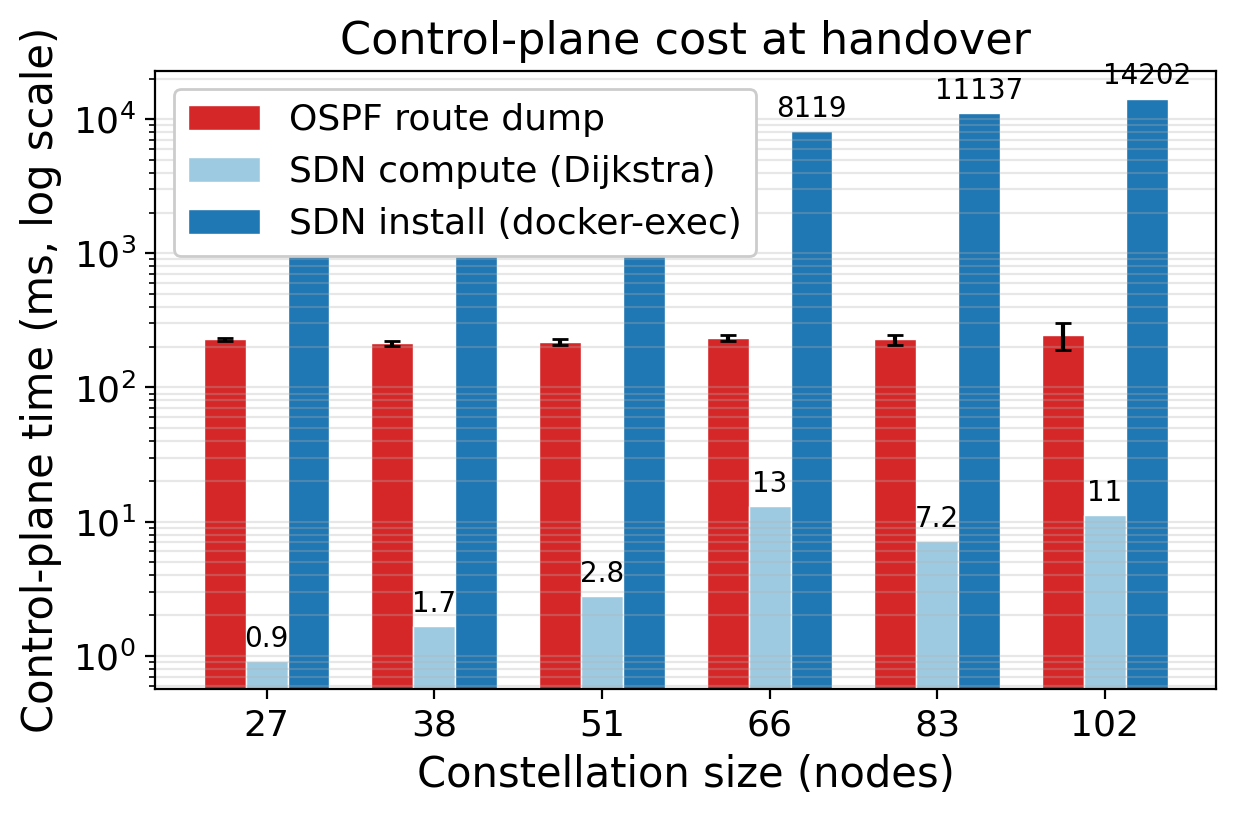
\includegraphics[width=\linewidth]{figures/control_handover.png}
  \caption{Control-plane time at the first handover (log scale).
    OSPF bars show BIRD route-dump collection (${\sim}200$–$230$\,ms).
    OrbitGraph splits algorithmic \texttt{compute\_ms} (Dijkstra, ${\sim}1$–$12$\,ms)
    from \texttt{install\_ms} (kernel route push via \texttt{docker exec},
    ${\sim}3.5$–$14.6$\,s at handover on large grids).}
  \label{fig:control-handover}
\end{figure}

\begin{figure}[!t]
  \centering
  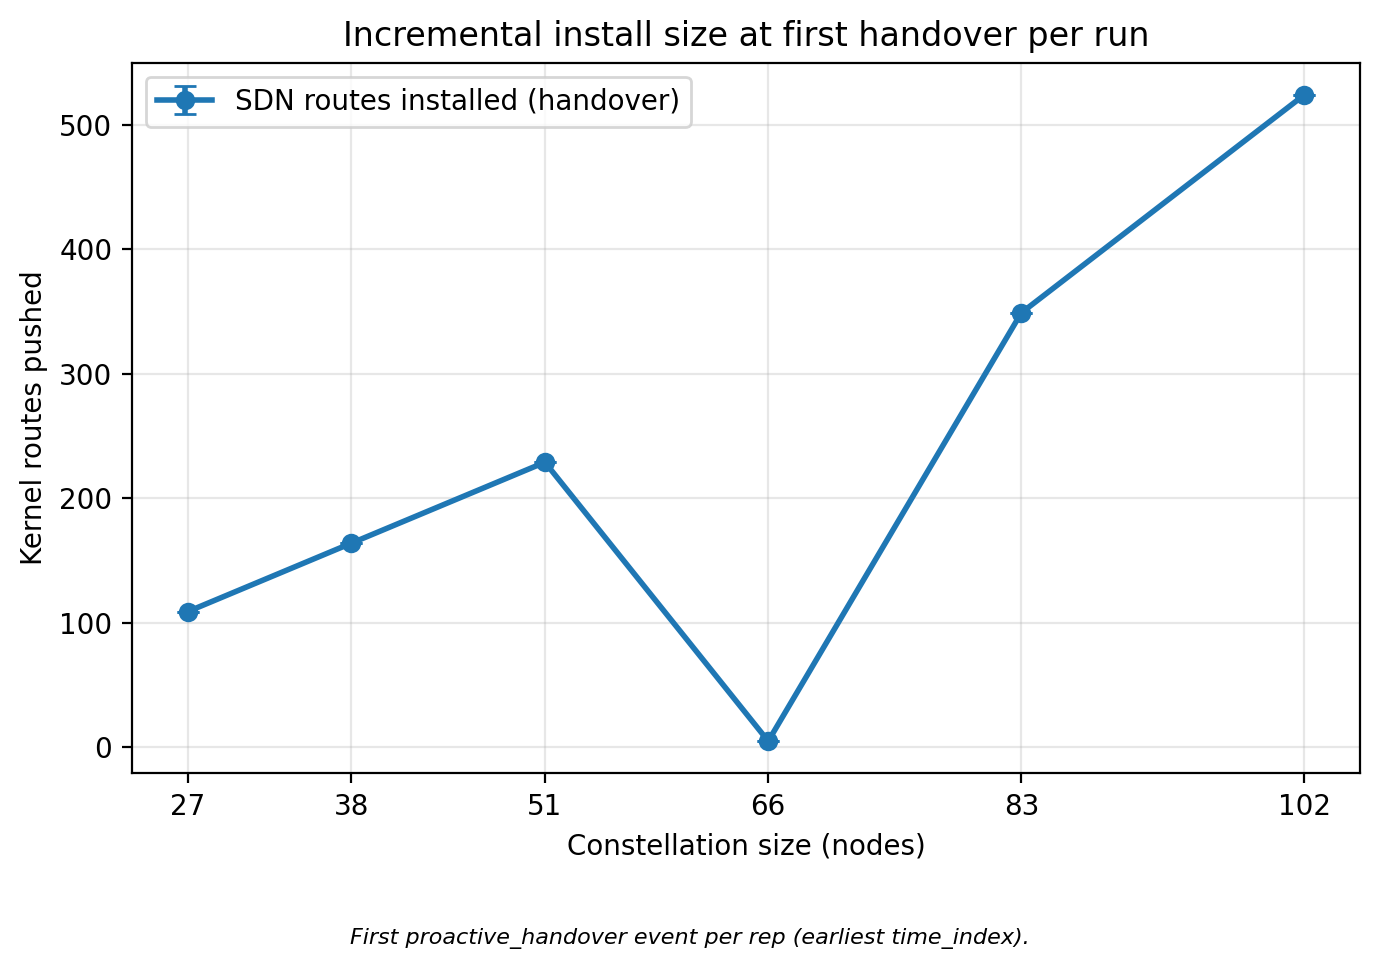
\includegraphics[width=\linewidth]{figures/routes_installed_handover.png}
  \caption{Kernel routes pushed at the first proactive handover (SDN only,
    mean~$\pm$~stddev).
    Incremental install touches hundreds of entries, not the full FIB
    (${\sim}10{,}504$ routes at $10{\times}10$ initialization).}
  \label{fig:routes-handover}
\end{figure}

Figure~\ref{fig:control-handover} separates control-plane \emph{algorithm} from
\emph{dataplane programming}.
OrbitGraph's graph recomputation remains in the \textbf{millisecond range}
(${\sim}0.9$–$12.7$\,ms across grids), confirming that shortest-path work on
$G_t$ is not the scalability bottleneck.
What dominates is \texttt{install\_ms}: pushing deltas through per-container
\texttt{docker exec} batches takes ${\sim}3.5$\,s on 27 nodes and
${\sim}14.6$\,s on 102 nodes at the first handover---orders of magnitude more
than OSPF's ${\sim}200$\,ms route \emph{observation} cost.

This asymmetry is intentional to report honestly.
OSPF's bar measures how long it takes to \emph{read} routing state after an
event; it does not include the multi-second reconvergence that
Figure~\ref{fig:outage-handover} shows in the data plane.
OrbitGraph's install bar is a \textbf{harness artifact} of our Docker southbound;
a production SDN plane (gRPC, NETCONF, or on-board agents receiving compressed
deltas) would shrink install time while preserving the same FIB semantics.

Crucially, heavy install does \emph{not} imply heavy data-plane outage when
updates are ordered proactively: the continuous probe in
Figure~\ref{fig:outage-handover} shows 0\,s black hole even while install runs,
because forwarding entries for the new path are already in place before the old
GSL disappears.

Figure~\ref{fig:routes-handover} explains \emph{why} install remains tractable.
Incremental deltas (Section~\ref{sec:incremental}) push only changed next-hops:
${\sim}109$ routes at the first handover on $5{\times}5$, rising to
${\sim}576$ on $10{\times}10$---roughly \textbf{20$\times$ fewer} programming
operations than the ${\sim}10{,}504$ routes required at initialization.
Without incremental install, every handover would replay a full-table push and
amplify the install-time penalty without improving availability.

\paragraph{Where the control plane is cheap.}
On delay-only ticks where next-hops are unchanged, OrbitGraph records
\texttt{fib\_unchanged} and skips the dataplane entirely
(${\sim}1$\,ms compute, zero install).
OSPF incurs no equivalent metric on these ticks, but also cannot proactively
reshape forwarding before a scheduled handover.

\subsection{Resilience under satellite failure}
\label{sec:analysis-damage}

\begin{figure}[!t]
  \centering
  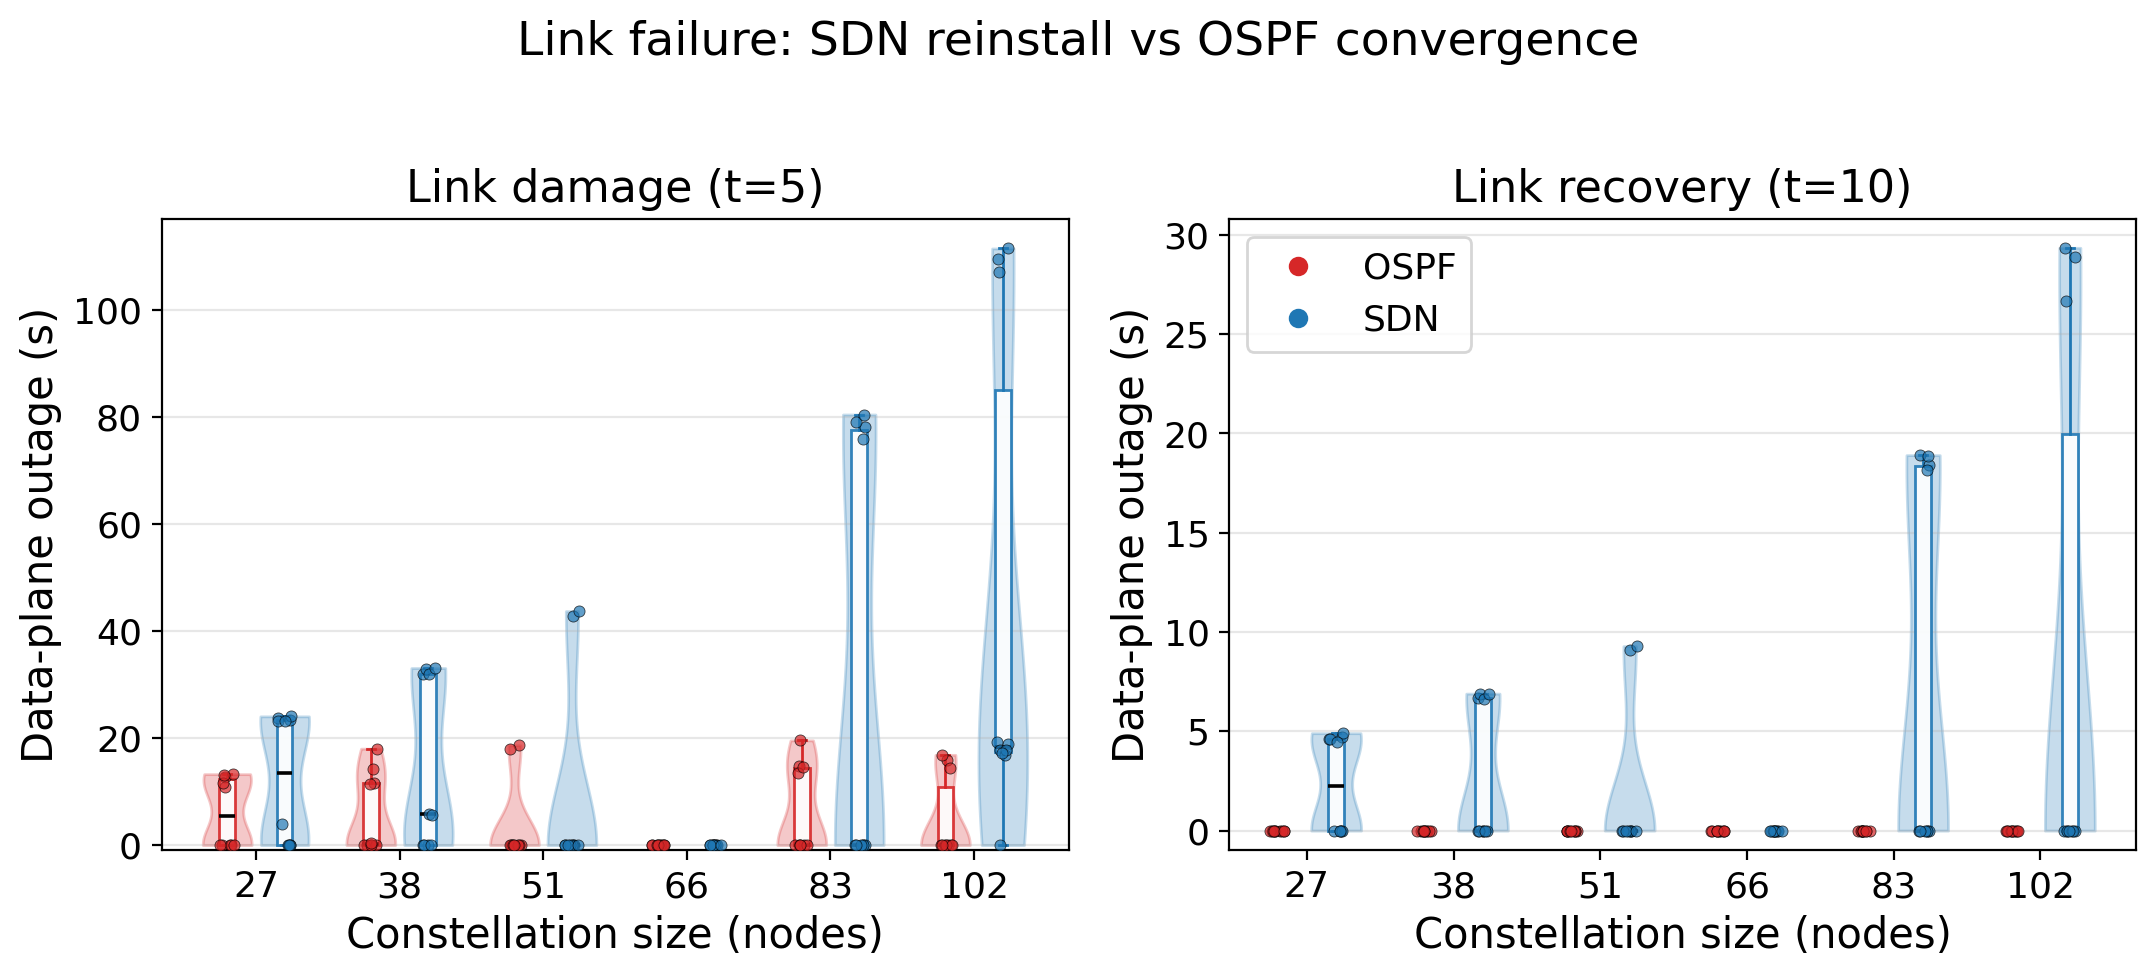
\includegraphics[width=\linewidth]{figures/outage_damage_recovery.png}
  \caption{Data-plane outage after link damage ($t{=}5$) and recovery ($t{=}10$),
    median per repetition.
    OrbitGraph does \emph{not} outperform OSPF on these events; SDN install
    latency can extend the loss burst relative to distributed reconvergence.}
  \label{fig:outage-damage}
\end{figure}

Figure~\ref{fig:outage-damage} presents a deliberately contrasting result---the
regime where OrbitGraph is \textbf{not} the better option today.

At $t{=}5$ we disable 30\% of satellites (100\% loss on all interfaces).
Both modes must recompute around a substantially changed $G_t$.
OrbitGraph reacts with a full incremental reinstall (\texttt{damage\_recovery}),
which blocks the synchronous emulation loop while thousands of routes are pushed.
Median data-plane outage for SDN \emph{exceeds} OSPF on several grids (e.g.,
${\sim}26$\,s vs.\ ${\sim}2.4$\,s median on 102 nodes in the aggregated cohort).

Three factors explain this gap:
\begin{enumerate}
  \item \textbf{No proactive ordering.} Unlike GSL handover, damage is a
        reactive event: links fail before the controller runs, so there is no
        make-before-break window at the topology level.
  \item \textbf{Large delta size.} Removing 30\% of satellites shifts many
        next-hops; the install set approaches a bulk update (${\sim}4{,}700$
        routes touched at 102 nodes) rather than the hundreds seen at handover.
  \item \textbf{Harness install path.} The same Docker exec southbound that
        Figure~\ref{fig:control-handover} shows at handover applies here without
        the compensating benefit of proactive link overlap.
\end{enumerate}

After recovery at $t{=}10$, both modes return to low outage on most grids;
neither maintains a decisive advantage.
For unplanned failures, distributed protocols that converge locally---or SDN
with a faster southbound and pipelined delta streaming---remain competitive
with centralized graph recomputation~\cite{gregory:satellite-routing:2022}.

This honest boundary clarifies OrbitGraph's sweet spot: \emph{scheduled,
orbit-predictable topology changes} (GSL handovers, planned ISL reconfiguration)
where global graph knowledge and update ordering translate directly into
zero-outage forwarding continuity.

\subsection{Summary of trade-offs}

Table~\ref{tab:tradeoffs} consolidates the analysis.
OrbitGraph's graph-centric SDN approach delivers its clearest win on the metric
operators care about for mega-constellation handover---end-to-end availability
during contact migration---while trading higher programmatic control-plane effort
(measurable but not user-visible when updates are proactive) and showing no
advantage under bulk failure injection with our current install path.

\begin{table}[!t]
  \centering
  \caption{OrbitGraph vs.\ OSPF: where SDN wins, ties, and lags.}
  \label{tab:tradeoffs}
  \renewcommand{\arraystretch}{1.12}
  \begin{tabular}{@{}p{0.22\linewidth}ccp{0.28\linewidth}@{}}
    \hline
    Scenario & OSPF & OrbitGraph & Comment \\
    \hline
    GSL handover outage      & Multi-second & \textbf{0\,ms} & Proactive install \\
    Handover/post-HO loss    & Up to 100\% & \textbf{0\%} & Fig.~\ref{fig:phase-metrics} \\
    Steady-state RTT         & Similar & Similar & Same LeastDelay paths \\
    Dijkstra compute         & n/a & \textbf{1–13\,ms} & Scales mildly \\
    Route push at handover   & n/a & ${\sim}10^2$–$10^3$ routes & vs.\ ${\sim}10^4$ init \\
    Satellite damage outage  & \textbf{Lower} & Higher & No proactive window \\
    Route-dump / observe     & \textbf{${\sim}200$\,ms} & n/a & Not reconvergence \\
    \hline
  \end{tabular}
\end{table}

In graph-centric terms, OrbitGraph treats each snapshot $G_t$ as a first-class
object: recomputation is cheap, deltas are small at handover, and update
\emph{timing} relative to link lifetime is the lever that SDN alone can pull.
Distributed OSPF remains a robust default for unplanned churn and for networks
without a trusted global view; OrbitGraph shows that when the LEO network \emph{is}
a dynamic graph with known handover schedules, centralized shortest-path control
can keep that graph connected in the data plane through every contact change.
